\chapter{E1-f}
\label{cha:E1f}

The E1-f run at Jefferson Lab operated from April through June of 2003.
The run used a 5.498 GeV electron beam with a 75.1$\pm$0.2\% polarization.
The target was unpolarized liquid hydrogen.
It was determined that running the torus magnet at 60\% of its maximum value would improve acceptance.
Both charged pion channels - $\pi^+$ and $\pi^-$ - were binned and studied in a fully differential way over a broad kinematic range ($0.1 < x < 0.6$, $1.0 < Q^2 < 4.7\ \text{GeV}^2$, $0.0 < z < 0.9$, $0.0 < P_{h\perp}^2 < 1.0\ \text{GeV}^2$, and $-180^\circ < \phi_h < 180^\circ$) within SIDIS kinematic cuts ($W > 2.05$ GeV, $y < 0.85$, and $Q^2 > 1.0\ \text{GeV}^2$) (see figure~\ref{fig:binningScheme}).
\begin{figure}[htp]
\centering
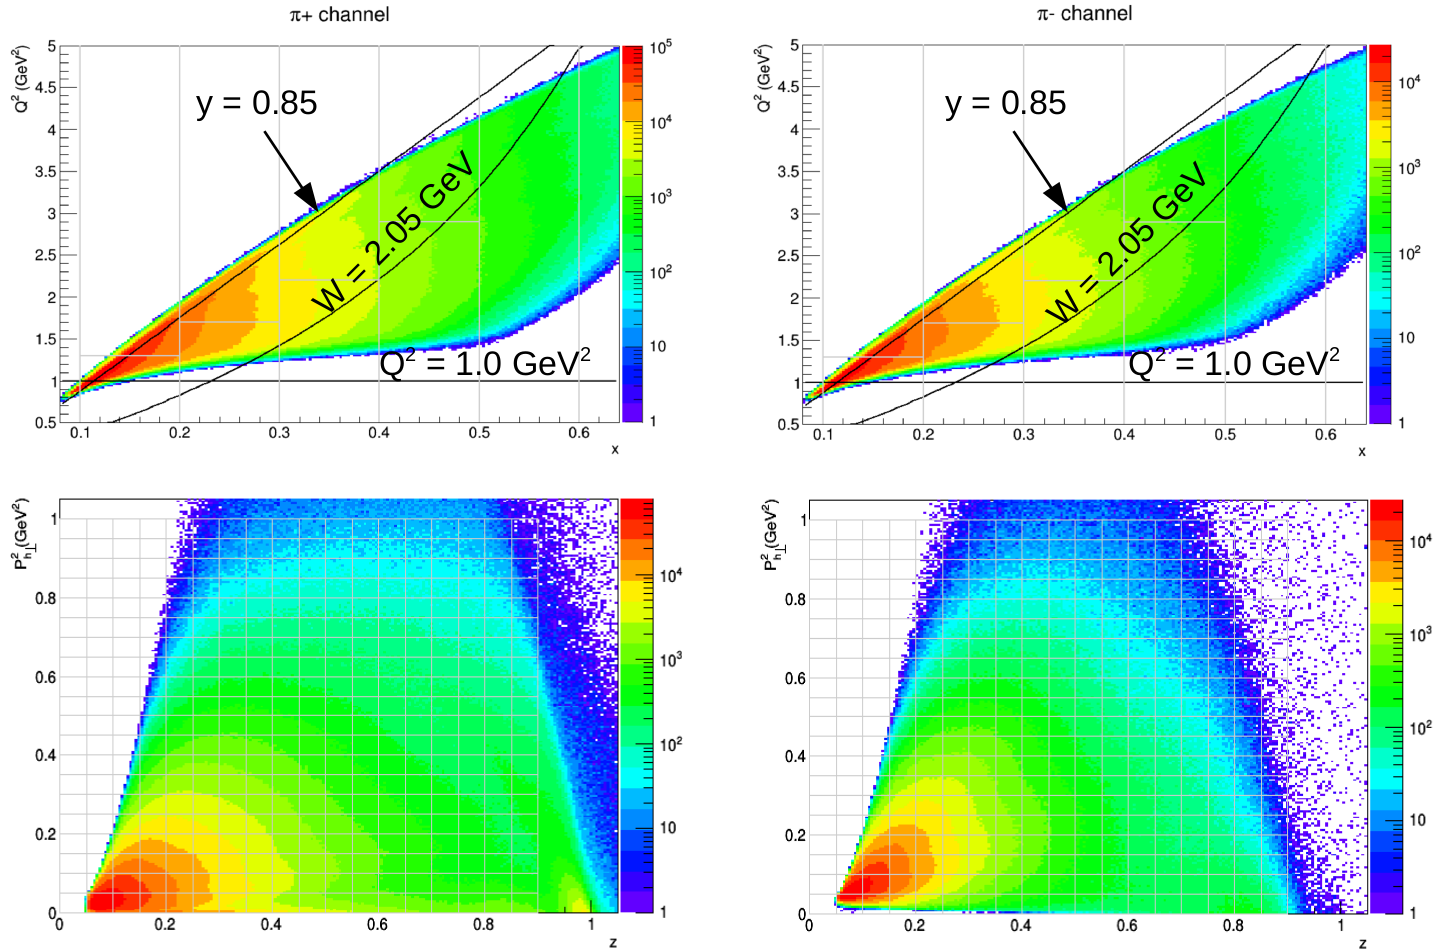
\includegraphics[width=4.5in]{figures/binningScheme.png}
\caption{The $x$-$Q^2$ (top) and $z$-$P_{h\perp}^2$ (bottom) kinematic coverage and binning scheme for $\pi^+$ (left) and $\pi^-$ (right) for the E1-f data set.}
\label{fig:binningScheme}
\end{figure}



